% $Header: svn+ssh://andre@crapman/home/junda/repos/andre/school/trunk/m/Chapter/stat/probability/chapter/prob.intro.tex 221 2021-02-13 18:18:09Z andre $
\tikzsetfigurename{ch.00.02.units}
% \tikzexternaldisable
% \tikzexternalenable

% \part{Kombi}
% \section{Intro}
\subsection*{\label{subsec0002.1_siUnit}SI-Einheiten}
%= = = = = = = = = = = = = = = = = = = = = = = = = = = = = = = = = = = = = = =
%= = = = = = = = = = = = = = = = = = = = = = = = = = = = = = = = = = = = = = =
% \iffalse
\begin{frame}
  \frametitle{SI-Einheiten}
  \framesubtitle{Das internationale Einheitensystem}
  %%= = = = = = = = = = = = = = = = = = = = = = = = = = = = = = = = = = = = = =
  \begin{block}{Messen - Gr\"o\ss{}en - Einheiten}
    \pause 
    Finden Sie heraus, wie folgende Einheiten definiert sind:\\
    \parbox[t]{0.30\linewidth}{
    \begin{itemize}
      \item <+-> Morgen (Fl\"ache)
      \item <+-> Elle (L\"ange)
      \item <+-> Meile (L\"ange)
      \item <+-> Pfund (Masse)
      \item <+-> Unze (Masse)
      \item <+-> Gallone (Volumen)
      \item <+-> Rie\ss{} (Volumen)
    \end{itemize}
    }\hspace{\stretch{1}}\parbox[t]{0.69\linewidth}{
    \ifteacher{%%
      \pause
      \begin{itemize}
        \item <+-> mit einem Ochsen am Vormittag pfl\"ugbare Fl\"ache
        \item <+-> Abstand Nase - Fingerspitze des
          gestreckten Arms
        \item <+-> u. a. 5000 Fuß, viele unterschiedliche Definitionen
        \item <+-> $\nicefrac{1}{2}$, 0,453\,592\,37 oder 373,241\,721\,6 kg
        \item <+-> $\nicefrac{1}{16}$ Pfund, 28,349\,523\,125 g
        \item <+-> 4,54609 l (UK), 3,78541 l (US)
        \item <+-> Menge Papier, die ein Esel tragen kann
           \\ heute: 480 oder 500 B\"ogen A4 Papier mit $\unitfrac[80]{g}{m^2}$
      \end{itemize}
    }
    \else{}\fi
    }
  \end{block}
  %%= = = = = = = = = = = = = = = = = = = = = = = = = = = = = = = = = = = = = =
\end{frame}
%==============================================================================

% \section{Intro}
% \subsection*{\label{subsec0002.1_siUnit}SI-Einheiten}
%= = = = = = = = = = = = = = = = = = = = = = = = = = = = = = = = = = = = = = =
%= = = = = = = = = = = = = = = = = = = = = = = = = = = = = = = = = = = = = = =
% \iffalse
\begin{frame}
  \frametitle{SI-Einheiten}
  \framesubtitle{Das internationale Einheitensystem}
  %%= = = = = = = = = = = = = = = = = = = = = = = = = = = = = = = = = = = = = =
  \begin{block}{Gr\"o\ss{}en und Einheiten}
    \pause 
    Physikalische Gr\"o\ss{}en sind messbare \adSTField[2]{Eigenschaften} von 
    Objekten, e. g. \adSTField[2]{L\"ange}, \adSTField[2]{Masse},
    \adSTField[2]{Zeit}, \adSTField[2]{Gewicht}, \adSTField[2]{elektrische
    Spannung}, \adSTField[2]{elektrische Stromst\"arke}, \dots
    \pause
    
    Physikalische \adSTField[2]{Einheiten} haben \adSTField[2]{definierte} 
    Werte f\"ur eine Gr\"o\ss{}e, z. B. \adSTField[2]{Meter} f\"ur
    \adSTField[2]{L\"ange}, \adSTField[2]{Kilogramm} f\"ur \adSTField[2]{Masse},
    \adSTField[2]{Sekunde} f\"ur \adSTField[2]{Zeit}, \dots
    
    \pause
    Mit genau definierten Einheiten k\"onnen Gr\"o\ss{}en an unterschiedlichen
    Orten und Zeiten \adSTField[2]{vergleichbar} gemacht werden. Manchmal 
    m\"ussen Gr\"o\ss{}en \adSTField[2]{umgerechnet} werden, z. B.
    \adSTField[2]{km/h} in \adSTField[2]{m/s}, oder \adSTField[2]{cm} in
    \adSTField[2]{Zoll}.

    \pause 
    Jede \adSTField[2]{Gr\"o\ss{}e} hat (mind.) ein \adSTField[2]{Symbol}, z. B.
    \adSTFieldm[2]{m} f\"ur \adSTField[2]{Masse}, \adSTFieldm[2]{t} f\"ur
    \adSTField[2]{Zeit}, \adSTFieldm[2]{F} f\"ur \adSTField[2]{Kraft}, \dots

    \pause 
    Jede \adSTField[2]{Einheit} hat auch eine Abk\"urzung, z. B.
    \adSTFieldm[2]{m} f\"ur \adSTField[2]{Meter}, \adSTFieldm[2]{s} f\"ur
    \adSTField[2]{Sekunde}, \adSTFieldm[2]{kg} f\"ur \adSTField[2]{Kilogramm}, \dots
  \end{block} 
  % \parbox[t]{0.2\linewidth}{
  % }\hspace{\stretch{1}}\parbox[t]{0.69\linewidth}{
  % }\\
  %%= = = = = = = = = = = = = = = = = = = = = = = = = = = = = = = = = = = = = =
\end{frame}
%==============================================================================

% \section{Intro}
% \subsection*{\label{subsec0002.1_siUnit}SI-Einheiten}
\ifteacher
%= = = = = = = = = = = = = = = = = = = = = = = = = = = = = = = = = = = = = = =
%= = = = = = = = = = = = = = = = = = = = = = = = = = = = = = = = = = = = = = =
% \iffalse
\begin{frame}
  \frametitle{SI-Einheiten}
  \framesubtitle{Das internationale Einheitensystem}
  %%= = = = = = = = = = = = = = = = = = = = = = = = = = = = = = = = = = = = = =
  \begin{block}{Vervollst\"andigen Sie die Tabelle}
    \pause 
    \begin{tabular}{@{}llll@{}}
      Gr\"o\ss{}e               & Symbol & Einheit   & Umrechnung \\ \hline
      L\"ange                   & $l$    & Meter     & 1 m = 100 cm = 1000 mm \\
      Masse                     & $m$    & Kilogramm & 1 kg = 1000 g = 1\,000\,000 mg \\
                                &        &           & 1 t = 1000 kg = 1\,000\,000 g \\
      Zeit                      & $t$    & Sekunde   & 1 min = 60 s; \\
                                &        &           & 1 h = 60 min = 3600 s \\
      L\"ange                   &  $l$  &  Meter      &  1 m  \\
      Masse       & $m$                &  Kilogramm  &  1 kg  \\
       Zeit        &  $t$  & Sekunde   &  1 s  \\
       Volumen     &  $V$  & Liter     &  1 L  \\
      Geschwindigkeit           &  $v$  &  Meter pro Sekunde  &  \unitfrac[1]{m}{s}  \\
       Beschleunigung  &  $a$  &  Meter pro Quadratsekunde  & $\unitfrac[1]{m}{s^2}$  \\
       Kraft          &  $F$  & Newton &  1 N \\
      elektrische Stromst\"arke & $I$    & Ampere    & 1 A = 1000 mA \\
      Temperatur                & $T$    & Kelvin    & K = ${^\circ}$C + 273,15 \\
      Stoffmenge                & $n$    & Mol       & mol\\
      Lichtst\"arke             & $J$    & Candela   & cd
    \end{tabular}
    
  \end{block}
  \parbox[t]{0.2\linewidth}{
  }\hspace{\stretch{1}}\parbox[t]{0.69\linewidth}{
  }\\
  %%= = = = = = = = = = = = = = = = = = = = = = = = = = = = = = = = = = = = = =
\end{frame}
%==============================================================================
\else
%= = = = = = = = = = = = = = = = = = = = = = = = = = = = = = = = = = = = = = =
% \iffalse
\begin{frame}
  \frametitle{SI-Einheiten}
  \framesubtitle{Das internationale Einheitensystem}
  %%= = = = = = = = = = = = = = = = = = = = = = = = = = = = = = = = = = = = = =
  \pause 
  \begin{block}{Vervollst\"andigen Sie die Tabelle}
    \begin{tabular}{@{}llll@{}}
      Gr\"o\ss{}e               & Symbol & Einheit   & Abk\"urzung \\ \hline
      L\"ange                   & \adSTField[2]{$l$} & \adSTField[2]{Meter}     & \adSTField[2]{1 m} \\
      \adSTField[2]{Masse}      & $m$                & \adSTField[2]{Kilogramm} & \adSTField[2]{1 kg} \\
      \adSTField[2]{Zeit}       & \adSTField[2]{$t$} & Sekunde   & \adSTField[2]{1 s} \\
      \adSTField[2]{Volumen}    & \adSTField[2]{$V$} & Liter     & \adSTField[2]{1 L} \\
      Geschwindigkeit           & \adSTField[2]{$v$} & \adSTField[2]{Meter pro Sekunde} & \adSTField[2]{\unitfrac[1]{m}{s}}\\
      \adSTField[2]{Beschleunigung} & \adSTField[2]{$a$} & \adSTField[2]{Meter pro Quadratsekunde} & \adSTFieldm[2]{\unitfrac[1]{m}{s^2}}\\
      \adSTField[2]{Kraft}         & \adSTField[2]{$F$} & Newton & \adSTField[2]{1 N} \\
      Temperatur                & \adSTField[2]{$T$}    & Kelvin    & K = ${^\circ}$C + 273,15 \\
    \end{tabular}
  \end{block}
  \parbox[t]{0.2\linewidth}{
    \ifteacher
      \rule[0pt]{0mm}{4\baselineskip}
    \else
      \rule[0pt]{0mm}{4\baselineskip}
    \fi

  }\hspace{\stretch{1}}\parbox[t]{0.69\linewidth}{
  }\\
  %%= = = = = = = = = = = = = = = = = = = = = = = = = = = = = = = = = = = = = =
\end{frame}
%==============================================================================
\fi

% \section{Intro}
% \subsection*{\label{subsec0002.1_siUnit}SI-Einheiten}
%= = = = = = = = = = = = = = = = = = = = = = = = = = = = = = = = = = = = = = =
%= = = = = = = = = = = = = = = = = = = = = = = = = = = = = = = = = = = = = = =
% \iffalse
\begin{frame}
  \frametitle{SI-Einheiten}
  \framesubtitle{Das internationale Einheitensystem}
  %%= = = = = = = = = = = = = = = = = = = = = = = = = = = = = = = = = = = = = =
    \pause
    \begin{block}{Einheitliche Einheiten}
    Das \adSTField[]{internationale Einheitensystem} (Système International
    d'Unités, SI) wurde 1960 von der 11. Generalkonferenz für Maß und Gewicht
    (CGPM) eingeführt, und ist heute das weltweit am meisten verwendete
    Einheitensystem. Es besteht aus sieben \adSTField[]{Basiseinheiten}, die
    alle anderen Einheiten lassen sich daraus ableiten.
    \pause
    \begin{itemize}
      \item <+-> Meter (m) - \adSTField[2]{L\"ange}
      \item <+-> Kilogramm (kg) - \adSTField[2]{Masse}
      \item <+-> Sekunde (s) - \adSTField[2]{Zeit}
      \item <+-> Ampere (A) - \adSTField[2]{elektrische Stromstärke}
      \item <+-> Kelvin (K) - \adSTField[2]{thermodynamische Temperatur}
      \item <+-> Mol (mol) - \adSTField[2]{Stoffmenge}
      \item <+-> Candela (cd) - \adSTField[2]{Lichtstärke}
    \end{itemize}
  \end{block} 
  \parbox[t]{0.2\linewidth}{
  }\hspace{\stretch{1}}\parbox[t]{0.69\linewidth}{
  }
  %%= = = = = = = = = = = = = = = = = = = = = = = = = = = = = = = = = = = = = =
\end{frame}
%==============================================================================

% \section{Intro}
\subsection*{\label{subsec0003.1_magnitude}Gr\"o\ss{}enordnungen}
%= = = = = = = = = = = = = = = = = = = = = = = = = = = = = = = = = = = = = = =
%= = = = = = = = = = = = = = = = = = = = = = = = = = = = = = = = = = = = = = =
% \iffalse
\begin{frame}
  \frametitle{Gr\"o\ss{}enordnungen}
  \framesubtitle{Prefixe und 10-er Potenzen}
  %%= = = = = = = = = = = = = = = = = = = = = = = = = = = = = = = = = = = = = =
  \begin{block}{Mikro bis Makro}
    \pause 
    \begin{itemize}
      \item <+-> Welche Masse besitzt die Erde? 
      \item <+-> Wie lang ist ein Lichtjahr? 
      \item <+-> Wie groß ist der Durchmesser eines Wasserstoffatoms?
      \item <+-> Wie viel wiegt ein Proton? 
      \item <+-> Wie lange dauert eine Nanosekunde?
    \end{itemize}
    \ifteacher
    \begin{itemize}
      \item <+-> 5\,970\,000\,000\,000\,000\,000\,000\,000 kg oder $5{,}97 \times 10^{24}$ kg 
      \item <+-> 9\,460\,000\,000\,000\,000 m oder $9{,}46 \times 10^{15}$ m 
      \item <+-> 0,000\,000\,000\,1 m oder $1 \times 10^{-10}$ m 
      \item <+-> 0,000\,000\,000\,000\,000\,000\,000\,000\,001\,67 kg $1{,}67 \times 10^{-27}$ kg 
      \item <+-> 0,000\,000\,001 s oder $1 \times 10^{-9}$ s 
    \end{itemize}
    }
    \else
    \rule[0pt]{0mm}{6\baselineskip}
    \fi
  \end{block} 
  \parbox[t]{0.2\linewidth}{
  }\hspace{\stretch{1}}\parbox[t]{0.69\linewidth}{
  }
  %%= = = = = = = = = = = = = = = = = = = = = = = = = = = = = = = = = = = = = =
\end{frame}
%==============================================================================

% \section{Intro}
% \subsection*{\label{subsec0003.1_magnitude}Gr\"o\ss{}enordnungen}
%= = = = = = = = = = = = = = = = = = = = = = = = = = = = = = = = = = = = = = =
%= = = = = = = = = = = = = = = = = = = = = = = = = = = = = = = = = = = = = = =
% \iffalse
\begin{frame}
  \frametitle{Gr\"o\ss{}enordnungen}
  \framesubtitle{Prefixe und 10-er Potenzen}
  %%= = = = = = = = = = = = = = = = = = = = = = = = = = = = = = = = = = = = = =
  \begin{block}{Von der Sch\"onheit von Zahlen}
    \pause
    Bei Gr\"o\ss{}en in der Natur kommen \adSTField[]{Zahlenwerte} vor, die mit
    vielen \adSTField[]{Nullen} dargestellt werden, und daher 
    \adSTField[2]{un\"ubersichtlich} sind. 
    \pause
    Man verwendet \adSTField[2]{10-er Potenzen}, um die Zahlen \"ubersichtlicher 
    anzuschreiben.
    \pause 
    Ebenso erleichern \adSTField[2]{Prefixe} die Lesbarkeit von Zahlen.
  \end{block} 
  \pause
  \begin{block}{10-er Potenzen}
    % \adRule{8}{5}%%
    \parbox[t]{0.23\linewidth}{%%
      \ifteacher%%
        \begin{array}[t]{@{}rrr@{}}
          n & 10^n & \text{Zahl}\tabularnewline
          \hline
          1 & 10^1 & 10 \tabularnewline
          2 & 10^2 & 100 \tabularnewline
          3 & 10^3 & 1000 \tabularnewline
          4 & 10^4 & 10\,000 \tabularnewline
          5 & 10^5 & 100\,000 \tabularnewline
            &&\dots\tabularnewline
          \hline
        \end{array}
      \else
        \begin{array}[t]{@{}rrr@{}}
          n & 10^n & \text{Zahl}\tabularnewline
          \hline
          1 & \fbox{\phantom{$10^1$}} & \fbox{\phantom{10      }} \tabularnewline
          2 & \fbox{\phantom{$10^2$}} & \fbox{\phantom{100     }} \tabularnewline
          3 & \fbox{\phantom{$10^3$}} & \fbox{\phantom{1000    }} \tabularnewline
          4 & \fbox{\phantom{$10^4$}} & \fbox{\phantom{10\,000 }} \tabularnewline
          5 & \fbox{\phantom{$10^5$}} & \fbox{\phantom{100\,000}} \tabularnewline
            &&\dots\tabularnewline
          \hline
        \end{array}
      \fi
    } 
    \ifteacher sowie \fi\pause
    \parbox[t]{0.23\linewidth}{%%
      \ifteacher%%
        \begin{array}[t]{@{}rrl@{}}
          n & 10^n & \text{Zahl}\tabularnewline
          \hline
          -1 & 10^{-1} & 0.1 \tabularnewline
          -2 & 10^{-2} & 0.01 \tabularnewline
          -3 & 10^{-3} & 0.001 \tabularnewline
          -4 & 10^{-4} & 0.000\,1 \tabularnewline
          -5 & 10^{-5} & 0.000\,01 \tabularnewline
            &&\dots\tabularnewline
          \hline
        \end{array}
      \else
        \begin{array}[t]{@{}rrr@{}}
          n & 10^n & \text{Zahl}\tabularnewline
          \hline
          -1 & \fbox{\phantom{$10^{-1}$}} & \fbox{\phantom{$0.1$}} \tabularnewline
          -2 & \fbox{\phantom{$10^{-2}$}} & \fbox{\phantom{$0.01$}} \tabularnewline
          -3 & \fbox{\phantom{$10^{-3}$}} & \fbox{\phantom{$0.001$}} \tabularnewline
          -4 & \fbox{\phantom{$10^{-4}$}} & \fbox{\phantom{$0.000\,1$}} \tabularnewline
          -5 & \fbox{\phantom{$10^{-5}$}} & \fbox{\phantom{$0.000\,01$}} \tabularnewline
            &&\dots\tabularnewline
          \hline
        \end{array}
      \fi
    } \pause
    \parbox[t]{0.42\linewidth}{%%
        Die Anzahl der \adSTField[2]{Nullen} in den 10-er Potenzen ist
        \begin{itemize}
          \item<+-> bei \adSTField[2]{positiven} Potenzen $n$ Nullen 
            nach der 1
          \item<+-> bei \adSTField[2]{negativen} Potenzen $n$ Nullen
            vor der 1, die Null vor dem Komma wird mitgez\"ahlt
        \end{itemize}
    }
  \end{block} 

  \parbox[t]{0.2\linewidth}{
  }\hspace{\stretch{1}}\parbox[t]{0.69\linewidth}{
  }
  %%= = = = = = = = = = = = = = = = = = = = = = = = = = = = = = = = = = = = = =
\end{frame}
%==============================================================================

% \section{Intro}
% \subsection*{\label{subsec0003.1_magnitude}Gr\"o\ss{}enordnungen}
%= = = = = = = = = = = = = = = = = = = = = = = = = = = = = = = = = = = = = = =
%= = = = = = = = = = = = = = = = = = = = = = = = = = = = = = = = = = = = = = =
% \iffalse
\begin{frame}
  \frametitle{Gr\"o\ss{}enordnungen}
  \framesubtitle{Prefixe und 10-er Potenzen}
  %%= = = = = = = = = = = = = = = = = = = = = = = = = = = = = = = = = = = = = =
  \begin{block}{Prefixe}
    \pause
    Prefixe sind Vorsilben, die vor eine Einheit gesetzt werden, um
    \adSTField[]{Vielfache} oder \adSTField[]{Bruchteile} dieser Einheit zu
    bezeichnen. 
    \pause
    Die Vielfachen und Bruchteile sind immer \adSTField[2]{Potenzen} von 10.
  \end{block} 
  \pause
  \begin{block}{Beispiele}
    \ifteacher{%%
    \begin{itemize}
      \item <+-> 1 Kilometer (km) = 1000 Meter (m) = $10^3$ m
      \item <+-> 1 Zentimeter (cm) = 0,01 Meter (m) = $10^{-2}$ m
      \item <+-> 1 Millisekunde (ms) = 0,001 Sekunden (s) = $10^{-3}$ s
      \item <+-> 1 Megahertz (MHz) = 1\,000\,000 Hertz (Hz) = $10^6$ Hz
      \item <+-> 1 Mikrogramm ($\mu$g) = 0,000\,001 Gramm (g) = $10^{-6}$ g
    \end{itemize}}
    \else
      \rule[0pt]{0mm}{8\baselineskip}
    \fi
  \end{block} 
  \parbox[t]{0.2\linewidth}{
  }\hspace{\stretch{1}}\parbox[t]{0.69\linewidth}{
  }
\end{frame}
%==============================================================================

% \section{Intro}
% \subsection*{\label{subsec0003.1_magnitude}Gr\"o\ss{}enordnungen}
%= = = = = = = = = = = = = = = = = = = = = = = = = = = = = = = = = = = = = = =
%= = = = = = = = = = = = = = = = = = = = = = = = = = = = = = = = = = = = = = =
% \iffalse
\begin{frame}
  \frametitle{Gr\"o\ss{}enordnungen}
  \framesubtitle{Prefixe und 10-er Potenzen}
  %%= = = = = = = = = = = = = = = = = = = = = = = = = = = = = = = = = = = = = =
  \begin{block}{Prefixe}
    \pause 
    \begin{tabular}{@{}l*{4}{@{\,}l}@{}}
      Name     & Symbol & Faktor       & 10-er       & Beispiel \tabularnewline
      &&&                                Potenz      &  \tabularnewline\hline
      Tera     & T      & 1\,000\,000\,000\,000 & $10^{12}$ & 1 TB = 1\,000\,000\,000\,000 B \tabularnewline
      Giga     & G      & 1\,000\,000\,000 & $10^{9}$      & 1 GHz = 1\,000\,000\,000 Hz \tabularnewline
      Mega     & M      & 1\,000\,000   & $10^{6}$            & 1 MW = 1\,000\,000 W \tabularnewline
      Kilo     & k      & 1\,000       & $10^3$            & 1 km = 1\,000 m \tabularnewline
      Hekto    & h      & 100         & $10^2$            & 1 hL = 100 L \tabularnewline
      Deka     & da     & 10          & $10^1$            & 1 dag = 10 g \tabularnewline
      (Einheit)&        & 1           & $10^0$            & 1 m = 1 m \tabularnewline
      Dezi     & d      & 0,1         & $10^{-1}$         & 1 dL = 0,1 L \tabularnewline
      Zenti    & c      & 0,01        & $10^{-2}$         & 1 cm = 0,01 m \tabularnewline
      Milli    & m      & 0,001       & $10^{-3}$         & 1 mg = 0,001 g \tabularnewline
      Mikro    & $\mu$  & 0,000\,001  & $10^{-6}$         & 1 $\mu$s = 0,000\,001 s \tabularnewline
      Nano     & n      & 0,000\,000\,001& $10^{-9}$      & 1 nm = 0,000\,000\,001 m \tabularnewline
      Pico     & p      & 0,000\,000\,000\,001& $10^{-12}$& 1 pF = 0,000\,000\,000\,001 F \tabularnewline
      % Femto    & f      & 0,000\,000\,000\,000\,001& $10^{-15}$& 1 fs = 0,000\,000\,000\,000\,001 s \tabularnewline
      % Atto     & a      & 0,000\,000\,000\,000\,000\,001& $10^{-18}$& 1 aJ = 0,000\,000\,000\,000\,000\,000\,001 J \tabularnewline
      % Zepto    & z      & 0,000\,000\,000\,000\,000\,000\,001& $10^{-21}$& 1 zW = 0,000\,000\,000\,000\,000\,000\,000\,000\,001 W \tabularnewline
      % Yocto    & y      & 0,000\,000\,000\,000\,000\,000\,000\,000\,000\,001& $10^{-24}$& 1 yC = 0,000\,000\,000\,000\,000\,000\,000\,000\,000\,000\,000\,001 C \tabularnewline
      \hline
    \end{tabular}
  \end{block} 
  %%= = = = = = = = = = = = = = = = = = = = = = = = = = = = = = = = = = = = = =
\end{frame}
%==============================================================================

% \section{Intro}
% \subsection*{Naturwissenschaftliche Arbeitsweisen}
%= = = = = = = = = = = = = = = = = = = = = = = = = = = = = = = = = = = = = = =
%= = = = = = = = = = = = = = = = = = = = = = = = = = = = = = = = = = = = = = =
% \iffalse
\begin{frame}
  \frametitle{Naturwissenschaftliche Arbeitsweisen}
  \framesubtitle{Vom Fallen}
  %%= = = = = = = = = = = = = = = = = = = = = = = = = = = = = = = = = = = = = =
  
  Lange Zeit glaubte man, dass schwere K\"orper schneller fallen als leichte.
  Wie kann das \ifteacher{}widerlegt\else\fbox{\phantom{widerlegt}}\fi{}
  oder \ifteacher{}best\"atigt\else\fbox{\phantom{best\"atigt}}\fi{} werden?
  \pause
  \visible<+->{
    \begin{block}{Gedankenexperiment}
      \parbox[t]{0.3\linewidth}{
        \raisebox{\dimexpr-1.2\height+\ht\strutbox}{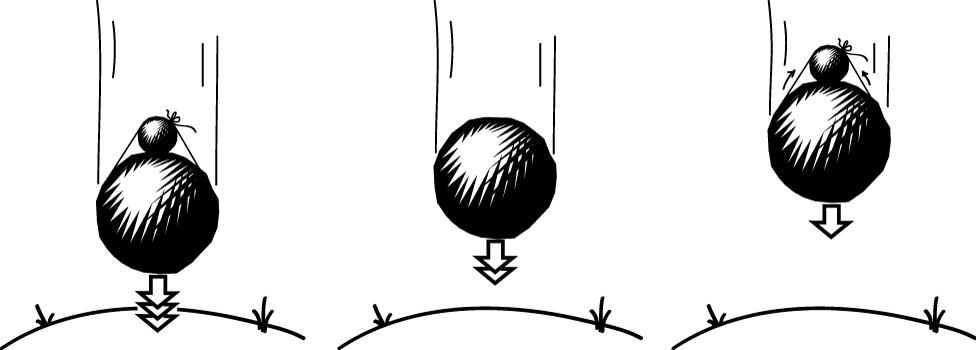
\includegraphics[width=0.98\linewidth]{./chapter/00.intro/pics/fallingStones.png}}\\
        {\tiny \url{https://personal.lse.ac.uk/robert49/ebooks/philsciadventures/img/balls2.gif}}
      }\hspace{\stretch{1}}\parbox[t]{0.69\linewidth}{
       \begin{itemize}
         \item<+-> \textbf{links}: Gro\ss{}er und kleiner Stein zusammen w\"urden
           \ifteacher{}schneller\else\fbox{\phantom{schneller}}\fi{}
           fallen (Aristoteles) als 
         \item<+-> \textbf{mitte}: der gro\ss{}e Stein alleine fallen w\"urde.
         \item <+-> \textbf{rechts}: der kleine Stein f\"allt laut Aristoteles
           \ifteacher{}langsamer\else\fbox{\phantom{langsamer}}\fi{} als der
           gro\ss{}e Stein, und w\"urde daher den gro\ss{}en Stein bremsen.
       \end{itemize}
      }
      \visible<+->{Das f\"uhrt zu einem \adSTField[1]{Widerspruch} zu Aristoteles,
      und veranlasste \adSTField[]{Galileo Galilei} zu der Annahme, dass
      alle K\"orper \adSTField[]{gleichschnell} fallen.}
    \end{block}
  }
  %%= = = = = = = = = = = = = = = = = = = = = = = = = = = = = = = = = = = = = =
\end{frame}
%==============================================================================

% \section{Intro}
% \subsection*{Naturwissenschaftliche Arbeitsweisen}
%= = = = = = = = = = = = = = = = = = = = = = = = = = = = = = = = = = = = = = =
%= = = = = = = = = = = = = = = = = = = = = = = = = = = = = = = = = = = = = = =
% \iffalse
\begin{frame}
  \frametitle{Naturwissenschaftliche Arbeitsweisen}
  \framesubtitle{Das Experiment}
  %%= = = = = = = = = = = = = = = = = = = = = = = = = = = = = = = = = = = = = =
  \parbox[t]{0.3\linewidth}{
    \raisebox{\dimexpr-1\height+\ht\strutbox}{%%
      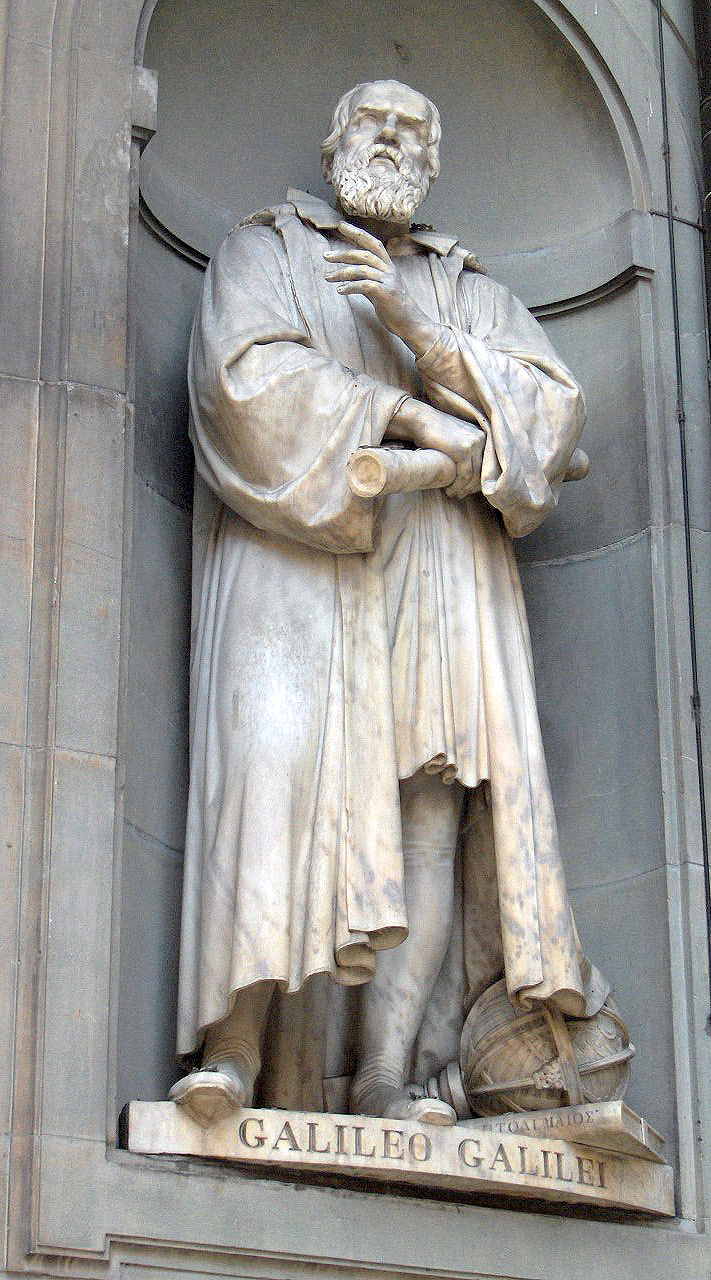
\includegraphics[width=0.75\linewidth]{./chapter/00.intro/pics/Galileo_Galilei01.png}}\\
    {\tiny Von User:JoJan - Eigenes Werk, CC BY-SA 3.0, 
     \url{https://commons.wikimedia.org/w/index.php?curid=408982}
     \url{https://commons.wikimedia.org/wiki/File:Galileo_Galilei_2.jpg}}
  }\hspace{\stretch{1}}\parbox[t]{0.69\linewidth}{
  \adSTField[]{Galileo Galilei} f\"uhrte \adSTField[]{falsifizierbare} 
    Experimente ein, und begr\"undet damit die \adSTField[]{moderne 
    Naturwissenschaft}.
  \pause
  Aus einer \adSTField[2]{Behauptung} (Hypothese) wird ein
  \adSTField[2]{Experiment} abgeleitet, das die Hypothese
  \adSTField[2]{widerlegen} (falsifizieren) kann.\pause{} Wird durch 
  Experimente die Hypothese nicht widerlegt, so ist sie
  \adSTField[2]{best\"atigt}, aber nicht bewiesen, und wird 
  zu einer \adSTField[2]{Theorie} erhoben. 
  \pause 
  Von Galileo Galilei stammt auch der Ausspruch:
  \pause
  \begin{quote}
    {Alles, was messbar ist, messen, \\
    alles was nicht messbar ist, 
    messbar machen.}
  \end{quote}
  \pause 
  Nach \adSTField[1]{Sir Karl Raimund Popper} ist eine Theorie nur dann
  \adSTField[1]{wissenschaftlich}, wenn sie \adSTField[1]{falsifizierbar} ist.
 }
  %%= = = = = = = = = = = = = = = = = = = = = = = = = = = = = = = = = = = = = =
\end{frame}
%==============================================================================

% % \section{Intro}
% % \subsection*{Naturwissenschaftliche Arbeitsweisen}
% %= = = = = = = = = = = = = = = = = = = = = = = = = = = = = = = = = = = = = = =
% %= = = = = = = = = = = = = = = = = = = = = = = = = = = = = = = = = = = = = = =
% % \iffalse
% \begin{frame}
%   \frametitle{Naturwissenschaftliche Arbeitsweisen}
%   \framesubtitle{Reference}
%   %%= = = = = = = = = = = = = = = = = = = = = = = = = = = = = = = = = = = = = =
% {
% \printbibliography[segment=\therefsegment,heading=subbib]
% % \printbibliography[segment=\therefsegment,heading=subbibliography,title={Online Sources}]
% }
% \end{frame}
% %==============================================================================

% % \section{Intro}
% \subsection*{Intro}
% %= = = = = = = = = = = = = = = = = = = = = = = = = = = = = = = = = = = = = = =
% %= = = = = = = = = = = = = = = = = = = = = = = = = = = = = = = = = = = = = = =
% % \iffalse
% \begin{frame}
%   \frametitle{Modelle}
%   \framesubtitle{Settings}
% %  \framesubtitle{Settings I}
%   %%= = = = = = = = = = = = = = = = = = = = = = = = = = = = = = = = = = = = = =
%
% \begin{block}{Settings I}
%   Die Kugeln werden nach der Ziehung
%   \begin{description}
%     \item [wieder zur\"uckgelegt]: der Ball kann daher \"ofter
%         gezogen werden, oder
%     \item [zur Seite gelegt]: dann wird der Ball maximal
%   einmal gezogen.
%   \end{description}
% \end{block}
%
% \pause
% \begin{block}{Settings II}
%   In der Urne befinden sich Kugeln, die
%   \begin{description}
%     \item [unterscheidbar sind]: jeder Ball ist ein Unikat (Farbe, Nummer,
%         Material, \dots)
%     \item [nicht unterscheidbar sind]: es gibt B\"alle, die die gleichen
%         Eigenschaften haben (z.~B. drei blaue und zwei rote B\"alle)
%   \end{description}
% \end{block}
%
% \end{frame}
% %==============================================================================
%
% % \section{Intro}
% % \subsection*{Modelle}
% %= = = = = = = = = = = = = = = = = = = = = = = = = = = = = = = = = = = = = = =
% %= = = = = = = = = = = = = = = = = = = = = = = = = = = = = = = = = = = = = = =
% % \iffalse
% \begin{frame}
%   \frametitle{Modelle}
%   \framesubtitle{Settings}
%   %%= = = = = = = = = = = = = = = = = = = = = = = = = = = = = = = = = = = = = =
%
% \begin{block}{Settings III}
%   Aus einer Urne mit $n$ Kugeln werden $k$ B\"alle gezogen.
%   \begin{description}
%     \item [$k=n$]: Permutationen
%     \item [$k<n$]: Variationen (alle B\"alle sind unterscheidbar)
%       und Kombinationen (B\"alle mit gleichen Eigenschaften)
%   \end{description}
% \end{block}
%
% \pause
% Aus wikipedia {\tiny(\url{https://de.wikipedia.org/wiki/Abz\%C3\%A4hlende_Kombinatorik\#Begriffsabgrenzungen})}:\\
% % https://de.wikipedia.org/wiki/Abz%C3%A4hlende_Kombinatorik#Begriffsabgrenzungen
% {\tiny
% Aufgrund der Vielfalt der Herangehensweisen sind die Schreibweisen und
% Begrifflichkeiten im Bereich der Kombinatorik leider oft recht uneinheitlich.
% Zwar bezeichnen übereinstimmend alle Autoren die Vertauschung der Reihenfolge
% einer Menge von $n$ unterscheidbaren Elementen als Permutation. W\"ahlt man
% dagegen von diesen $n$ Elementen nur $k < n$  Elemente aus, deren Reihenfolge
% man anschließend vertauscht, bezeichnen viele Autoren das nun als Variation,
% geordnete Stichprobe bzw. Kombination mit Berücksichtigung der Reihenfolge,
% andere dagegen (namentlich im englischsprachigen Raum) weiter als Permutation.
% L\"asst man schließlich in einer solchen Auswahl von Elementen deren
% Reihenfolge au\ss{}er Acht, wird solch eine Auswahl nun für gew\"ohnlich
% ungeordnete Stichprobe, Kombination ohne Berücksichtigung der Reihenfolge
% oder einfach nur Kombination genannt. Kombinationen sind also, sofern
% nichts weiter zu ihnen gesagt wird, in der Regel ungeordnet, Permutationen
% und/oder Variationen dagegen geordnet, wobei die Frage, ob man Permutationen
% als Sonderf\"alle von Variationen (oder umgekehrt) betrachtet, gegebenenfalls
% von Autor zu Autor unterschiedlich beantwortet wird.\\
% Alles in allem gibt es also zunächst einmal drei (oder auch nur zwei)
% verschiedene Fragestellungen, die ihrerseits noch einmal danach unterteilt
% werden, ob es unter den ausgewählten Elementen auch Wiederholungen gleicher
% Elemente geben darf oder nicht. Ist ersteres der Fall, spricht man von
% Kombinationen, Variationen oder Permutationen mit Wiederholung, andernfalls
% solchen ohne Wiederholung. Stellt man sich schließlich vor, dass die
% ausgew\"ahlten Elemente dabei einer Urne oder Ähnlichem entnommen werden,
% wird dementsprechend auch von Stichproben mit oder ohne Zur\"ucklegen
% gesprochen.\\
% }
%
% \end{frame}
% %==============================================================================
